\documentclass[12pt,a4paper]{article}

% Packages for formatting
\usepackage{geometry}
\geometry{a4paper, margin=1in}
\usepackage[utf8]{inputenc}
\usepackage{graphicx}
\usepackage{float}
\usepackage{subfig}
\usepackage{amsmath,amsfonts,amssymb}
\usepackage{booktabs}
\usepackage{caption}
\usepackage{subcaption}

% Begin document
\begin{document}

% Title page
\begin{titlepage}
    \centering
    \vspace*{0cm}
    \Huge{\textbf{Alarm Clock Development Project}}\\
    \Large{University of South Carolina}\\
    \Large{Department of Mechanical Engineering}\\

    \vspace{18cm}
    \normalsize{Graed R. Exampel}\\
    \vspace{0.1cm}
    \normalsize{March 16, 2024}\\
    \vspace{0.5cm}
    \normalsize{EMCH 368, Mechatronics}\\
    \vspace{0.1cm}
    \normalsize{Professor: Dr. Nikolaos Vitzilaois}\\
    \vfill
\end{titlepage}

\newpage

% Introduction
\section{Introduction}
In today's schedule-driven world, effective time management is essential. Thus, this project aimed to develop not just any alarm clock, but a sophisticated time management tool. By integrating mechanical and electronic components, we've moved beyond traditional designs to offer a reliable, efficient, and highly functional alarm clock. Enhanced features include programmable alarms, customizable tones, and an easy-to-use interface, transforming the alarm clock into an indispensable aid for personal organization and punctuality.


\subsection{Thesis}
The primary objective of this project was the development of an efficient and reliable alarm clock. This was approached by investigating the synergistic integration of mechanical and electronic components, aiming to create a product that is not only effective in its basic function but also enhanced with additional features to aid users in time management. The project sought to address common shortcomings of existing alarm clocks, such as limited customization options, poor user interface, and unreliability, by employing advanced technology and innovative design principles. The resulting product was anticipated to set a new standard in the domain of personal time-keeping devices, demonstrating that with thoughtful design, an everyday object can be transformed into an essential tool for modern living.

\subsection{Possible Uses for the Product}
The alarm clock designed in this project transcends the conventional limitations of such devices, offering a range of applications beyond simply waking a person from sleep. In homes, it serves as a central element in managing daily schedules, ensuring that all family members start their day on time and adhere to their personal routines. In offices, it can be used to manage meeting schedules, break times, and work deadlines, fostering a culture of punctuality and efficiency. Educational institutions can leverage its capabilities to maintain class schedules, conduct timely examinations, and manage time effectively in various academic activities. Additionally, the customization features allow the alarm clock to be adapted to different environments and user needs, making it a versatile tool in the pursuit of structured and disciplined time management. This adaptability ensures that the alarm clock is not just a reactive device that signals the start of a day but a proactive partner in the user's daily life.

\newpage
\section{Material List}
The construction of the alarm clock utilized the following materials, each illustrated below:
\begin{itemize}
    \item (1) Arduino Uno Microprocessor (Fig.~\ref{fig:arduino})
    \item (10) Jumper wires (Fig.~\ref{fig:jumperwires})
    \item (1) Breadboard (Fig.~\ref{fig:breadboard})
    \item (6) LED lights (Fig.~\ref{fig:ledlights})
    \item (1) Piezo Buzzer (Fig.~\ref{fig:piezobuzzer})
    \item (7) Resistors (Fig.~\ref{fig:resistor})
    \item (1) Push buttons (Fig.~\ref{fig:pushbuttons})
\end{itemize}

% Photos of Materials
\section{Photos of Materials}
Below are the materials used in the project:

\begin{figure}[H]
    \centering
    \subfloat[Arduino Uno Microprocessor]{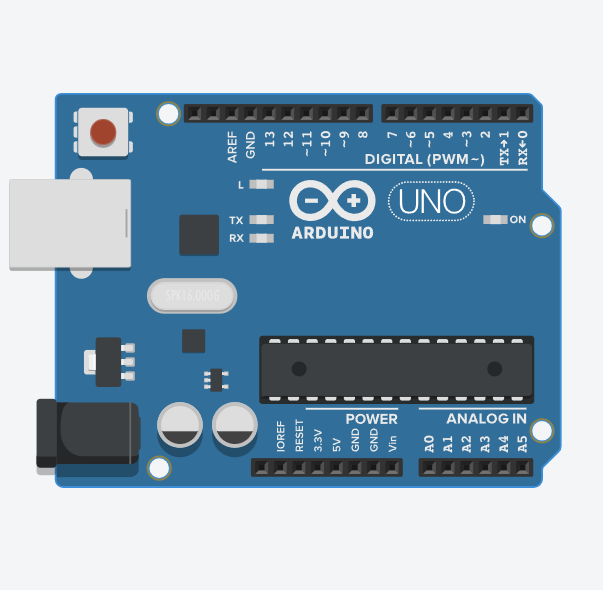
\includegraphics[width=3.5cm]{arduino_uno.png} \label{fig:arduino}}
    \subfloat[Jumper wires]{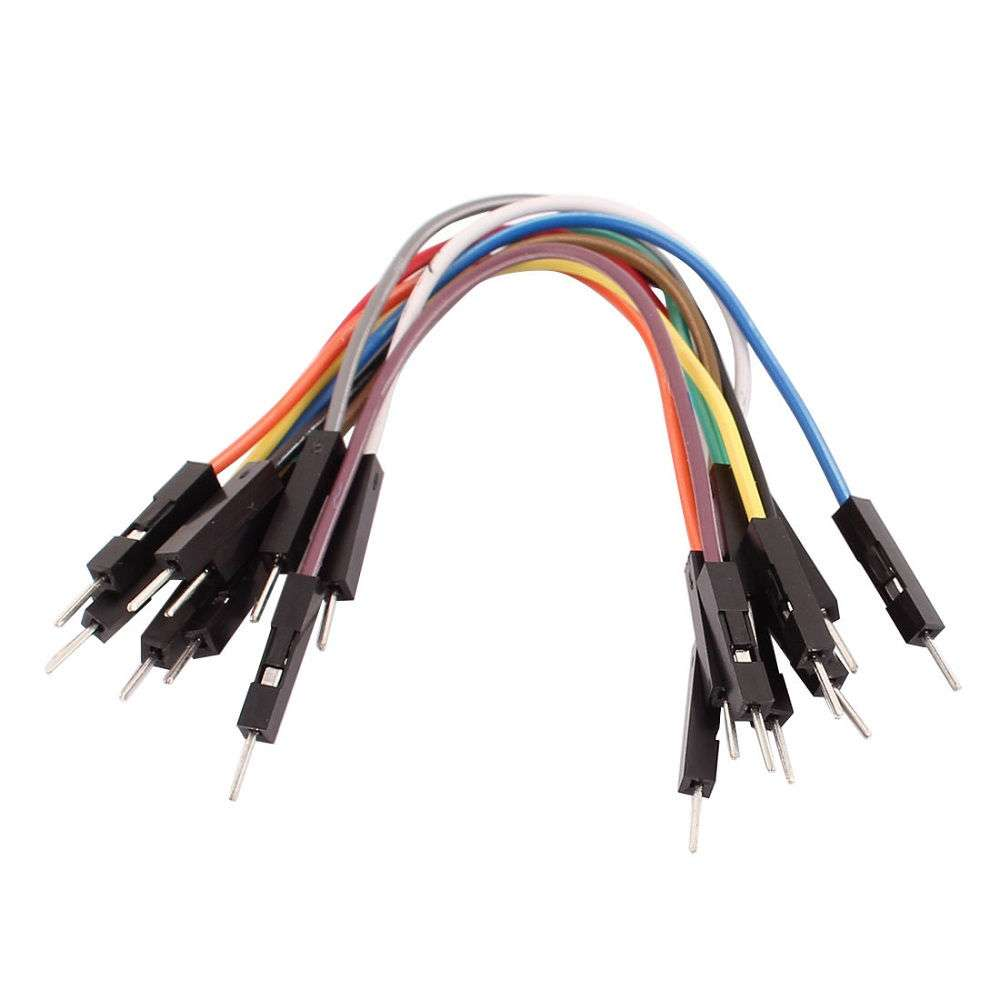
\includegraphics[width=3.5cm]{jumpers.jpg} \label{fig:jumperwires}}
    \subfloat[Breadboard]{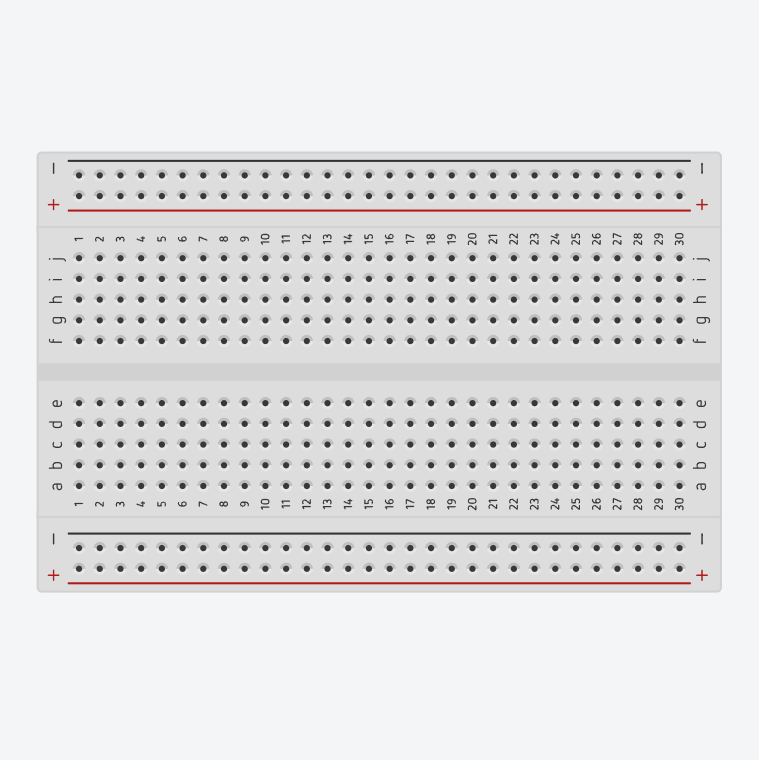
\includegraphics[width=3.5cm]{breadboard.png} \label{fig:breadboard}}
    \subfloat[LED lights]{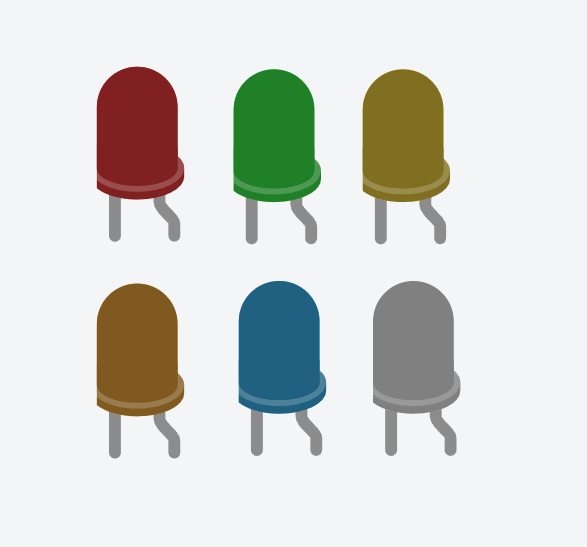
\includegraphics[width=3.5cm]{led_lights.png} \label{fig:ledlights}}\\
    \subfloat[Piezo Buzzer]{
\includegraphics[width=3.5cm]{piezo_buzzer.png} \label{fig:piezobuzzer}}
    \subfloat[Resistors]{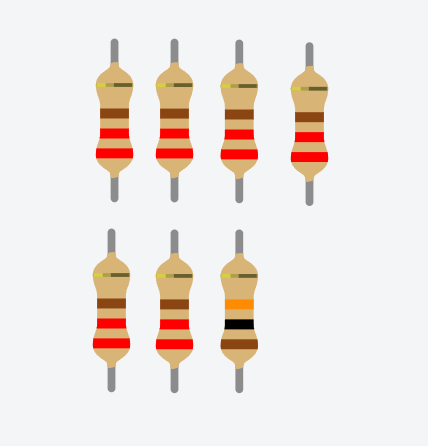
\includegraphics[width=3.5cm]{resistor.png} \label{fig:resistor}}
    \subfloat[Push buttons]{
\includegraphics[width=3.5cm]{push_buttons.png} \label{fig:pushbuttons}}
    \caption{Materials used in the alarm clock project.}
\end{figure}

\section{Selection Rationale}
\subsection{Arduino Uno Microprocessor}
The Arduino Uno was chosen for its balance of performance, ease of use, and cost. While alternatives like the Raspberry Pi offer higher processing power, the Uno's simplicity and extensive community support make it ideal for this introductory project.

\subsection{Jumper Wires}
Jumper wires were selected for their versatility and ease of use compared to permanent solder connections. Their color-coding aids circuit troubleshooting and learning, outweighing options like direct soldering, which lacks flexibility for beginners.

\subsection{Breadboard}
The use of a breadboard facilitates easy modifications and debugging. Alternatives such as PCBs provide permanence but lack the educational value of allowing students to experiment with circuit layouts easily.

\subsection{LED lights}
LEDs were chosen for their efficiency and visibility over traditional bulbs. Alternatives like incandescent bulbs were considered but dismissed due to higher power consumption and heat generation. The color variety of LEDs enhances user interaction and function indication.

\subsection{Piezo Buzzer}
The piezo buzzer was selected over other sound-producing components like speakers due to its compactness, lower power requirements, and clear sound output. While speakers could offer a wider range of sounds, the simplicity and efficiency of piezo buzzers are more suited to this project's scale and purpose.

\subsection{Resistors}
220 Ohm resistors were chosen to ensure LED longevity and proper operation. Other values were evaluated, but 220 Ohms provide the optimal balance between brightness and safety for the LEDs used in this project.

\subsection{Push Buttons}
Push buttons were favored for their straightforward functionality and feedback. Alternatives like touch sensors offer a modern approach but lack the tactile response beneficial for educational purposes and simplicity in circuit design.


% Photos - Complete Circuit
\section{Photos - Complete Circuit}
\begin{figure}[H]
    \centering
    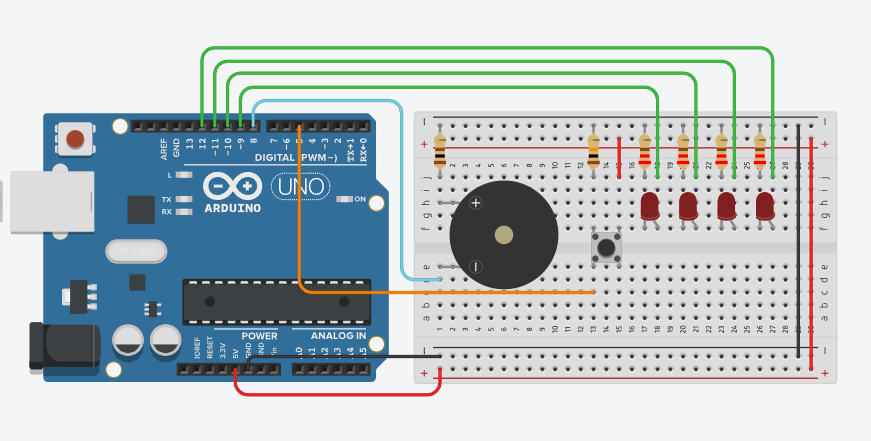
\includegraphics[width=15cm]{complete_circuit.png}
    \caption{Completed circuit layout of the alarm clock project.}
\end{figure}

% Building Procedure
\section{Building Procedure}
The assembly of the alarm clock involved the following steps:
\begin{enumerate}
    \item Secure the Arduino Uno on the breadboard.
    \item Connect LED lights to digital pins through 220 Ohm resistors.
    \item Attach the piezo buzzer to a digital pin and ground.
    \item Set up push buttons for setting time and alarm functions.
    \item Link all components with jumper wires according to the circuit diagram.
\end{enumerate}

\section{Circuit Explanation}
The circuit is centered around the Arduino Uno, which processes inputs from push buttons to set and display time using LEDs and activate the piezo buzzer as an alarm. Users set the time and alarm through the buttons, while the Arduino tracks time internally. 
\newline

LEDs represent time units with distinct colors for hours and minutes, offering a clear visual indication of the time. When the alarm time matches the real time, the Arduino signals the piezo buzzer to emit an alarm sound, alerting the user.
\newline

The design employs a breadboard and jumper wires for an accessible and modifiable setup, ideal for educational purposes. Circuit functionality and behavior are determined by a C++ sketch on the Arduino, allowing for customization and teaching basic programming and electronic principles.


% Sketch Screenshot
\section{Sketch Screenshot [FAKE]}
\begin{figure}[H]
    \centering
    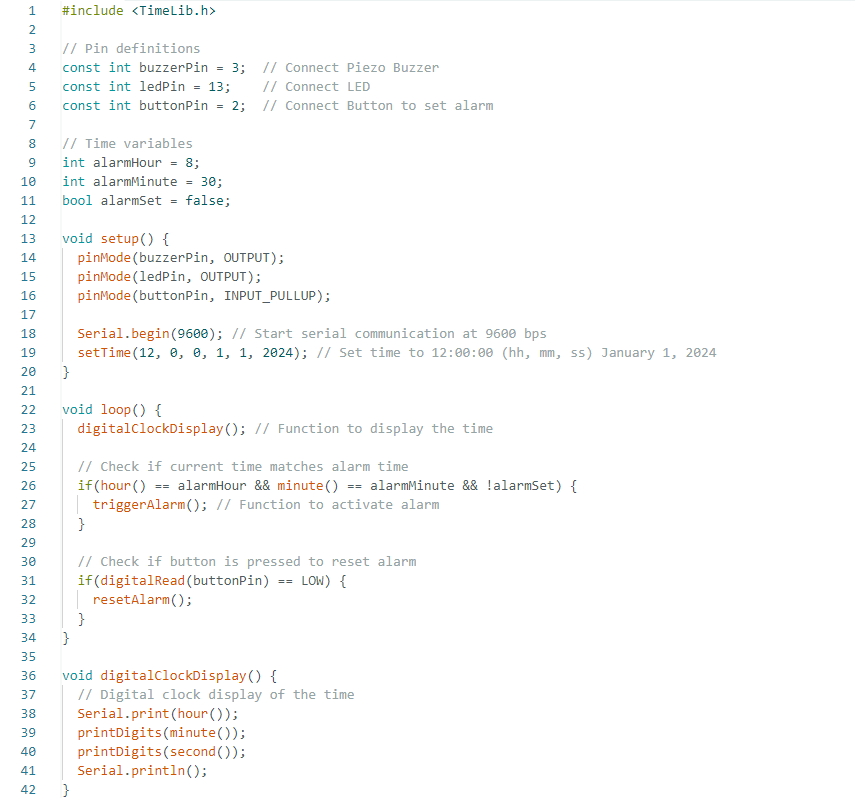
\includegraphics[width=16cm]{sketch_screenshot.png}
    \caption{Screenshot of the Arduino sketch used in the alarm clock project.}
\end{figure}

\section{Code Structure - Overall Breakdown}
The Arduino sketch is organized into distinct sections, each handling specific functionalities of the alarm clock. This modular structure facilitates easier understanding and debugging:

\begin{itemize}
    \item \textbf{setup():} Initializes the digital pins for input and output, begins serial communication, and sets the initial time. This function runs once when the program starts.
    \item \textbf{loop():} Represents the main program loop, updating the displayed time and monitoring for the alarm condition. This function runs repeatedly, forming the core of the program's functionality.
    \item \textbf{digitalClockDisplay():} Handles the formatting and display of the current time on the serial monitor. It breaks down the time into readable units (hours, minutes, seconds).
    \item \textbf{printDigits():} A helper function used by digitalClockDisplay() to format time components, ensuring two-digit representation with leading zeros if necessary.
    \item \textbf{triggerAlarm():} Activates the alarm mechanisms (buzzer and LED) when the current time matches the preset alarm time. This function encapsulates the alarm's response behavior.
    \item \textbf{resetAlarm():} Allows for the deactivation of the alarm and resetting its state, ensuring the system is ready for the next alarm trigger.
\end{itemize}


\section{Logical Flow of Code and Explanation}
The logical flow of the alarm clock code begins with the `setup()` function, which marks the starting point of the sketch. In this initial phase, digital pins connected to the LEDs, buzzer, and buttons are set to their designated modes (input or output). Serial communication is also initiated for time display on the computer's serial monitor, and the initial time is established. This function runs only once each time the Arduino is powered on or reset. Following the setup, the sketch enters a continuous loop through the `loop()` function. Within this loop, the current time is regularly updated and displayed. This function continually checks if the current time corresponds with the preset alarm time. If they match and the alarm has not previously been activated—to prevent repetitive triggering—the `triggerAlarm()` function is invoked. 
\newline

The `digitalClockDisplay()` and `printDigits()` functions collaboratively ensure the time is formatted and displayed clearly on the serial monitor. `digitalClockDisplay()` compiles the time into an easily understandable format, while `printDigits()` ensures that each part of the time (hours, minutes, seconds) is displayed with two digits, introducing a leading zero when needed, thus facilitating effortless time reading.
\newline

When the actual time aligns with the alarm time set within the code, the `triggerAlarm()` function gets called into action. This function engages the alarm by illuminating the LED and activating the buzzer, providing both visual and auditory notifications. This mechanism highlights the alarm's active phase, signaling the arrival of the predetermined wake-up time. If the user wishes to deactivate the alarm, the `resetAlarm()` function is engaged by pressing the reset button. This action extinguishes the LED and silences the buzzer, thus terminating the alarm signal and reverting the alarm status to inactive. This reset prepares the system for the next cycle, conforming to the user-defined settings.
\newline

Furthermore, the continuous operation of the `loop()` function enables real-time monitoring and interaction. The code reacts to changes such as the pressing of buttons for time setting or alarm resetting, assuring that the alarm clock remains both responsive and user-centric. This dynamic allows for direct user interaction, like adjusting the time or turning off the alarm, rendering the device both interactive and user-friendly. Through this cyclic and interactive approach, the code effectively manages the various functionalities of the alarm clock, catering to the users' needs while also providing an educational insight into programming and electronic design.

\section{Conclusion}
The Alarm Clock Development Project represents a successful fusion of mechanical and electronic engineering principles aimed at addressing real-world challenges in time management and personal organization. Throughout this project, from conceptualization to realization, a user-centric design was maintained, ensuring the final product not only meets the basic requirements of an alarm clock but also extends its utility through customizable features and an intuitive interface.

\end{document}
